% ============================================================================
% monografia.tex - Bayesian Universal Stochastic Differential Equations
%                  for ENSO Dynamics, Forecasting, and Parameter Sensitivity
%
% Monografía - Licenciatura en Ciencia de Datos (LCD), UBA
% Curso: Datos en Ecuaciones Diferenciales e Inteligencia Artificial (DEDIA)
% ============================================================================

\documentclass[11pt,a4paper]{article}

% ── Encoding & Language ──────────────────────────────────────────────────────
\usepackage[utf8]{inputenc}
\usepackage[T1]{fontenc}
\usepackage[spanish,es-tabla]{babel}

% ── Mathematics ──────────────────────────────────────────────────────────────
\usepackage{amsmath,amssymb,amsfonts,amsthm}

% ── Typography ───────────────────────────────────────────────────────────────
\usepackage{lmodern}
\usepackage{microtype}

% ── Layout & Geometry ────────────────────────────────────────────────────────
\usepackage[margin=2.5cm]{geometry}
\usepackage{setspace}
\onehalfspacing

% ── Figures & Tables ─────────────────────────────────────────────────────────
\usepackage{graphicx}
\usepackage{float}
\usepackage{booktabs}
\usepackage{caption}
\usepackage{subcaption}
\captionsetup{font=small,labelfont=bf}

% ── References & Links ───────────────────────────────────────────────────────
\usepackage[round,authoryear]{natbib}
\usepackage[colorlinks=true,linkcolor=blue!70!black,citecolor=blue!70!black,urlcolor=blue!60!black]{hyperref}
\usepackage{url}

% ── Misc ─────────────────────────────────────────────────────────────────────
\usepackage{enumitem}
\usepackage{xcolor}

% ── Custom Commands ──────────────────────────────────────────────────────────
\newcommand{\R}{\mathbb{R}}
\newcommand{\E}{\mathbb{E}}
\newcommand{\KL}{\mathrm{KL}}
\newcommand{\ELBO}{\mathcal{L}_{\text{ELBO}}}
\newcommand{\Dt}{\Delta t}
\DeclareMathOperator{\Cov}{Cov}
\DeclareMathOperator{\Var}{Var}
\DeclareMathOperator{\RMSE}{RMSE}
\DeclareMathOperator{\CRPS}{CRPS}

% ============================================================================
% Title
% ============================================================================

\title{%
  \textbf{Ecuaciones Diferenciales Estocásticas Universales Bayesianas\\
  para la Dinámica, Predicción y Análisis de Sensibilidad del ENSO}
}

\author{%
  Proyecto Final --- Licenciatura en Ciencia de Datos (LCD)\\
  \textit{Datos en Ecuaciones Diferenciales e Inteligencia Artificial}\\[2mm]
  Facultad de Ciencias Exactas y Naturales\\
  Universidad de Buenos Aires\\[2mm]
  \texttt{mathiasrolando@gmail.com}
}

\date{Junio 2026}

\begin{document}
\maketitle

\begin{abstract}
El fenómeno de El Niño--Oscilación del Sur (ENSO) es el modo dominante de variabilidad climática interanual, con impactos socioeconómicos a escala global. Los modelos lineales tradicionales, como el Oscilador de Recarga de \citet{jin1997}, capturan la escala temporal fundamental del ENSO pero no logran representar las no-linealidades observadas ni la irregularidad temporal de los eventos extremos. En este trabajo se presenta un marco de \textbf{Ecuaciones Diferenciales Estocásticas Universales Bayesianas (BUSDE)} que combina un esqueleto físico informado con correcciones aprendidas mediante redes neuronales, estimación variacional de parámetros, y un modelo de ruido estocástico dependiente del estado para capturar la incertidumbre aleatoria. Se entrena el modelo en datos mensuales del índice Niño 3.4 (SST, ERSSTv5) y del volumen de agua caliente (WWV) durante 1980--2010, y evaluamos su desempeño fuera de muestra en 2011--2021 utilizando métricas determinísticas (RMSE, correlación) y probabilísticas (CRPS, Brier Score, cobertura de intervalos de predicción). Los resultados demuestran que el modelo BUSDE supera al baseline climatológico en horizontes cortos (1–3 meses) con mejoras estadísticamente significativas, y mantiene skill positivo hasta 6 meses, y que las correcciones neuronales aprenden dinámicas físicamente interpretables. Se discuten las limitaciones del marco, incluyendo la subdispersión observada en horizontes largos y las restricciones estadísticas del periodo de prueba.
\end{abstract}

\vspace{3mm}
\noindent\textbf{Palabras clave:} ENSO, ecuaciones diferenciales estocásticas, aprendizaje científico de máquina, inferencia bayesiana, redes neuronales universales, predicción probabilística.

% ============================================================================
% 1. INTRODUCCIÓN
% ============================================================================
\section{Introducción}
\label{sec:introduccion}

El fenómeno de El Niño--Oscilación del Sur (ENSO) constituye el modo dominante de variabilidad climática interanual en el sistema acoplado océano-atmósfera del Pacífico tropical \citep{mcphaden2006}. Los eventos de El Niño y La Niña producen anomalías en la temperatura superficial del mar (SST) de hasta $\pm 2.5\,^{\circ}\mathrm{C}$ en la región Niño~3.4 ($5^{\circ}\mathrm{S}$--$5^{\circ}\mathrm{N}$, $170^{\circ}\mathrm{W}$--$120^{\circ}\mathrm{W}$; \citealt{trenberth1997}), con consecuencias económicas, agrícolas y ecológicas a escala planetaria.

La complejidad del ENSO radica en la coexistencia de una dinámica oscilatoria cuasi-periódica con una marcada irregularidad temporal. El espectro de potencia exhibe un pico dominante en la banda de 2--7 años, pero el intervalo entre eventos sucesivos muestra un coeficiente de variación (CV $= \sigma / \mu$) elevado, inconsistente con un oscilador periódico puro \citep{timmermann2018}. Esta irregularidad ha sido atribuida a la interacción entre dinámicas determinísticas no-lineales (asimetrías El Niño/La Niña, retroalimentación evaporativa) y forzamiento estocástico externo, particularmente las ráfagas de viento del oeste (\textit{Westerly Wind Bursts}, WWB; \citealt{eisenman2005}).

\subsection{Modelos físicos y sus limitaciones}

El Oscilador de Recarga (\textit{Recharge Oscillator}, RO) propuesto por \citet{jin1997} constituye el modelo conceptual de referencia para la dinámica del ENSO. Este modelo acopla la anomalía de SST ($T$) con el volumen de agua caliente ($h$, proxy de la profundidad de la termoclina) mediante un sistema lineal de dos ecuaciones:
\begin{equation}
\label{eq:ro_general}
\frac{dT}{dt} = aT + bh, \qquad
\frac{dh}{dt} = -cT + dh.
\end{equation}
La imposición de la restricción de \textbf{traza cero} ($\mathrm{Tr}(\mathbf{A}) = a + d = 0$, es decir, $d = -a$) garantiza la estabilidad neutral del oscilador, reduciendo el sistema a tres parámetros libres:
\begin{equation}
\label{eq:ro_intro}
\frac{dT}{dt} = aT + bh, \qquad
\frac{dh}{dt} = -cT - ah.
\end{equation}
Si bien este modelo captura el periodo fundamental del ENSO ($\approx 3$--5 años), su naturaleza lineal le impide representar las asimetrías observadas entre El Niño (calentamiento rápido e intenso) y La Niña (enfriamiento lento y moderado), así como la irregularidad temporal de los eventos.

\subsection{Ecuaciones diferenciales universales}

Las Ecuaciones Diferenciales Universales (UDE; \citealt{rackauckas2020}) ofrecen un paradigma para combinar modelos físicos con aprendizaje automático. En una UDE, un esqueleto dinámico conocido se aumenta con correcciones parametrizadas por redes neuronales, permitiendo que el modelo ``aprenda'' las dinámicas no representadas a partir de los datos. Este enfoque ha mostrado resultados prometedores en diversas aplicaciones científicas \citep{chen2018}.

\subsection{Objetivos de este trabajo}

En este trabajo desarrollamos un marco de \textbf{Ecuaciones Diferenciales Estocásticas Universales Bayesianas (BUSDE)} para ENSO que:
\begin{enumerate}[label=(\roman*)]
  \item Aumenta el Oscilador de Recarga con correcciones neuronales para capturar no-linealidades físicas.
  \item Estima distribuciones posteriores sobre los parámetros mediante inferencia variacional (Bayes-by-Backprop; \citealt{blundell2015}).
  \item Incorpora ruido estocástico dependiente del estado para representar la incertidumbre aleatoria.
  \item Produce pronósticos probabilísticos evaluados con métricas de calibración rigurosas.
\end{enumerate}

% ============================================================================
% 2. MÉTODOS
% ============================================================================
\section{Métodos}
\label{sec:metodos}

\subsection{Datos}
\label{sec:datos}

Utilizamos dos series temporales mensuales alineadas sobre el periodo común 1980--2021:
\begin{itemize}
  \item \textbf{SST (variable $T$):} Anomalía de temperatura superficial del mar en la región Niño~3.4, calculada a partir del dataset ERSSTv5 (\textit{Extended Reconstructed SST}, versión 5; \citealt{huang2017}). Las anomalías se computan respecto a la climatología mensual estricta del periodo de entrenamiento 1980--2010, evitando cualquier fuga de información del periodo de prueba.
  \item \textbf{WWV (variable $h$):} Anomalía del Volumen de Agua Caliente (\textit{Warm Water Volume}) del Pacífico ecuatorial, obtenida del NOAA Pacific Marine Environmental Laboratory (PMEL; \citealt{meinen2000}). Esta variable actúa como proxy de la profundidad de la termoclina y también se calibra para tener media cero en 1980--2010.
\end{itemize}

El periodo de entrenamiento abarca 1980--2010 ($N = 372$ observaciones mensuales) y el periodo de evaluación fuera de muestra comprende 2011--2021 ($N_{\text{test}} = 132$ meses). Las desviaciones estándar de las series de entrenamiento son $\sigma_T \approx 0.79\,^{\circ}\mathrm{C}$ y $\sigma_h \approx 1.44 \times 10^{14}\,\mathrm{m}^3$, valores utilizados como factores de normalización en la función de pérdida.

\subsection{Modelo baseline: Oscilador de Recarga lineal}
\label{sec:baseline}

Como referencia, ajustamos el RO lineal (Ec.~\ref{eq:ro_intro}) mediante Mínimos Cuadrados Ordinarios (OLS) sobre diferencias finitas centrales. Dado un conjunto de $N$ observaciones equiespaciadas con paso $\Dt = 1/12$ años, las derivadas se aproximan como:
\begin{equation}
\dot{T}_i \approx \frac{T_{i+1} - T_{i-1}}{2\Dt}, \qquad
\dot{h}_i \approx \frac{h_{i+1} - h_{i-1}}{2\Dt},
\end{equation}

para $i = 2, \ldots, N-1$. La restricción de traza cero reduce el sistema a tres parámetros libres ($a$, $b$, $c$), que se estiman por regresión lineal estándar. Los valores ajustados son $a = -0.237\,\text{año}^{-1}$, $b = 1.041\,\text{año}^{-1}$, $c = 3.162\,\text{año}^{-1}$, con un periodo natural $T_{\text{nat}} = 2\pi/\sqrt{bc} \approx 3.46$ años, consistente con la banda espectral dominante del ENSO. La simulación determinística se realiza con el integrador Tsit5 (Runge-Kutta 4/5) del ecosistema DifferentialEquations.jl \citep{rackauckas2017}.

\subsection{Ecuación Diferencial Estocástica Universal Bayesiana (BUSDE)}
\label{sec:busde}

El sistema BUSDE aumenta el RO con correcciones neuronales $f_\phi$ y $g_\phi$, y difusión estocástica:
\begin{align}
dT_t &= \Big[\underbrace{aT_t + bh_t}_{\text{RO lineal}} + \underbrace{f_\phi(T_t, h_t)}_{\text{corrección NN}}\Big]\,dt + \sigma_T(T_t, h_t)\,dW_{T,t}, \label{eq:busde_T} \\
dh_t &= \Big[-cT_t - ah_t + g_\phi(T_t, h_t) \Big]\,dt + \sigma_h(T_t, h_t)\,dW_{h,t}, \label{eq:busde_h}
\end{align}
donde $W_{T,t}$ y $W_{h,t}$ son procesos de Wiener independientes.

\subsubsection{Restricciones físicas}

Se imponen las siguientes restricciones para garantizar la consistencia física:
\begin{enumerate}[label=(\alph*)]
  \item \textbf{Traza cero:} $d = -a$, asegurando oscilación neutral.
  \item \textbf{Signos de acoplamiento:} $b > 0$ y $c > 0$, parametrizados como $b = e^{\log b}$ y $c = e^{\log c}$.
  \item \textbf{Amortiguamiento acotado:} $a \in [-0.40, -0.05]\,\text{año}^{-1}$ (clamp tras cada paso de optimización).
\end{enumerate}

\subsubsection{Redes neuronales y características}

Las funciones $f_\phi$ y $g_\phi$ son redes feedforward de dos capas implementadas en Lux.jl \citep{lux2022}:
\begin{equation}
f_\phi, g_\phi: \R^5 \to \R, \qquad
\mathbf{x} = \left(\frac{T}{\sigma_T},\; \frac{h}{\sigma_h},\; \frac{T^2}{\sigma_T^2},\; \frac{h^2}{\sigma_h^2},\; \frac{Th}{\sigma_T \sigma_h}\right)^{\!\top},
\end{equation}
con arquitectura $5 \to 16\;(\tanh) \to 1\;(\text{lineal})$. La capa de salida se inicializa con pesos pequeños (${\sim \mathcal{N}(0, 10^{-4})}$) para garantizar que las correcciones neuronales comiencen cerca de cero, preservando el esqueleto físico durante las primeras iteraciones de entrenamiento.



\subsubsection{Integración numérica}

Se utiliza un esquema simpléctico de Euler-Cromer \citep{cromer1981} que actualiza $T$ primero y luego $h$ usando el valor actualizado $T_{t+1}$:
\begin{align}
T_{t+1} &= T_t + \Dt\,\text{Drift}_T(T_t, h_t) + \sigma_T(T_t, h_t)\,\Delta W_T, \label{eq:euler_T}\\
h_{t+1} &= h_t + \Dt\,\text{Drift}_h(T_{t+1}, h_t) + \sigma_h(T_{t+1}, h_t)\,\Delta W_h, \label{eq:euler_h}
\end{align}
donde $\Delta W \sim \mathcal{N}(0, \Dt)$. Si bien el esquema de Euler-Cromer es formalmente simpléctico solo para sistemas hamiltonianos determinísticos, se usa aquí por la consistencia con el drift y la estabilidad numérica observada en simulaciones de largo plazo (500 años).


\subsubsection{Multiple Shooting}
\label{sec:ms}

Para estabilizar el cálculo de gradientes a través de trayectorias caóticas, empleamos la técnica de \textit{multiple shooting} \citep{bock1984}. Se definen ventanas de $W = 36$ meses (3~años) con un paso de $S = 6$ meses, generando múltiples segmentos superpuestos. Cada ventana se integra desde la condición inicial observada:
\begin{equation}
\mathcal{L}_{\text{MS}}(\theta) = \frac{1}{|\mathcal{W}|} \sum_{s \in \mathcal{W}} \frac{1}{W-1} \sum_{k=1}^{W-1} \left[\left(\frac{T_{s+k}^{\text{pred}} - T_{s+k}^{\text{obs}}}{\sigma_T}\right)^{\!2} + \left(\frac{h_{s+k}^{\text{pred}} - h_{s+k}^{\text{obs}}}{\sigma_h}\right)^{\!2}\right],
\end{equation}
donde $\mathcal{W}$ denota el conjunto de índices de inicio de las ventanas.

El truco de reparametrización $\theta = \mu + e^\rho \odot \varepsilon$, con $\varepsilon \sim \mathcal{N}(0, I)$, permite el cálculo eficiente de gradientes mediante diferenciación automática. La optimización se realiza con Adam durante 1000 iteraciones totales donde las primeras 600 se realizan con tasa de aprendizaje que luego se reduce a $3\times 10^{-4}$ para las últimas 400.


\subsubsection{Inferencia variacional: Bayes-by-Backprop}
\label{sec:bbb}

Siguiendo a \citet{blundell2015}, se modela la distribución posterior de los parámetros $\theta = \{a, \log b, \log c, \phi_f, \phi_g\}$ como una distribución gaussiana factorizada:
\begin{equation}
q(\theta \mid \mu, \rho) = \mathcal{N}\!\left(\mu,\; \text{diag}\big(e^{2\rho}\big)\right),
\end{equation}
donde $\mu$ y $\rho$ son parámetros variacionales. El prior es $p(\theta) = \mathcal{N}(0, \sigma_{\text{prior}}^2 I)$ con $\sigma_{\text{prior}} = 2.0$ para parámetros lineales y $\sigma_{\text{prior}} = 0.5$ para pesos de la red neuronal. Estas elecciones de prior se realizaron de forma heurística. Los parámetros se obtienen minimizando la pérdida variacional\footnote{Siguiendo la convención de \citet{blundell2015}, definimos $\ELBO$ como una función de \textit{pérdida} a minimizar (likelihood negativa + regularización KL). Nótese que esta convención invierte el signo respecto a la ELBO clásica de la inferencia variacional, que se maximiza.}:
\begin{equation}
\label{eq:elbo}
\ELBO(\mu, \rho) = \E_{q(\theta)}\!\left[\mathcal{L}_{\text{MS}}(\theta)\right] + \frac{1}{N}\,D_{\KL}\!\left(q(\theta \mid \mu, \rho) \,\|\, p(\theta)\right),
\end{equation}
donde $\mathcal{L}_{\text{MS}}$ es la pérdida de \textit{multiple shooting} y el factor $1/N$ escala la regularización de KL respecto al tamaño de los datos.



\subsubsection{Modelo de ruido estocástico}
\label{sec:noise}

Dado el modelo de drift entrenado (media posterior $\mu$), los residuos de predicción a un paso se definen como:
\begin{equation}
R_{T,t} = T_{t+1}^{\text{obs}} - T_{t+1}^{\text{pred}}, \qquad R_{h,t} = h_{t+1}^{\text{obs}} - h_{t+1}^{\text{pred}}.
\end{equation}
Bajo un SDE de Itô, estos residuos satisfacen $R \sim \mathcal{N}(0, \sigma^2 \Dt)$. Consideramos dos modelos de ruido:

\paragraph{Homoscedástico:} $\sigma_T = \text{std}(R_T)/\sqrt{\Dt}$, $\sigma_h = \text{std}(R_h)/\sqrt{\Dt}$ (constantes).

\paragraph{Heteroscedástico (dependiente del estado):}
\begin{equation}
\label{eq:hetero}
\sigma_T(T, h) = \exp(\gamma_{T,0} + \gamma_{T,1}\,T + \gamma_{T,2}\,h),
\end{equation}
cuyos parámetros $\gamma_T$ se estiman por máxima verosimilitud (MLE) sobre la densidad de transición gaussiana \citep{gardiner2009,kloeden1992}. Un modelo análogo se ajusta para $\sigma_h$. La optimización se realiza mediante el método de Nelder-Mead del paquete Optim.jl. Cabe destacar que el ruido se calibra \textbf{únicamente a un paso} ($\Delta t = 1/12$), lo cual es una limitación estructural para pronósticos a horizontes largos.

\subsection{Verificación probabilística}
\label{sec:verif}

Para evaluar la calidad de los pronósticos probabilísticos utilizamos:
\begin{itemize}
  \item \textbf{CRPS} (\textit{Continuous Ranked Probability Score}; \citealt{hersbach2000}): métrica que penaliza tanto el sesgo como la dispersión del ensamble. Calculamos el CRPS mediante el algoritmo eficiente $O(M \log M)$ de \citet{jordan2019}.
  \item \textbf{CRPSS} (\textit{CRPS Skill Score}): $\mathrm{CRPSS} = 1 - \mathrm{CRPS}_{\text{modelo}} / \mathrm{CRPS}_{\text{clima}}$, donde la climatología se computa estrictamente sobre el conjunto de entrenamiento para evitar el filtrado de información (\textit{data leakage}). Valores positivos indican superioridad respecto al baseline climatológico \citep{gneiting2007}.
  \item \textbf{Brier Score} (\citealt{brier1950}): $(p - o)^2$ para el evento binario ``El Niño'' ($T > 0.5\,^{\circ}\mathrm{C}$).
  \item \textbf{Cobertura del intervalo de predicción} al 90\%: fracción de observaciones contenidas entre los percentiles 5 y 95 del ensamble.
\end{itemize}

Los pronósticos probabilísticos combinan incertidumbre epistémica (muestreo de la distribución posterior de parámetros) con incertidumbre aleatoria (simulación estocástica de trayectorias SDE con ruido heteroscedástico), generando $M = 1000$ realizaciones por paso de inicio.

% ============================================================================
% 3. RESULTADOS
% ============================================================================





\section{Resultados}
\label{sec:resultados}

\subsection{Análisis exploratorio y baseline lineal}

El espectro de potencia del índice Niño~3.4 (método de Welch; \citealt{welch1967}) muestra un pico dominante en la banda de 2--7 años, confirmando la periodicidad cuasi-regular del ENSO. La distribución de intervalos entre eventos de El Niño (definidos por el criterio ONI: $T > 0.5\,^{\circ}\mathrm{C}$ durante $\geq 5$ meses consecutivos) exhibe un CV $\approx 0.46$, indicando una irregularidad sustancial que motiva el uso de modelos estocásticos.

El baseline lineal (RO ajustado por OLS) produce un RMSE de entrenamiento moderado, pero su simulación determinística de largo plazo diverge rápidamente de las observaciones ($r \approx 0.51$ en rollout sobre 2011--2021), confirmando la insuficiencia del modelo lineal para capturar la evolución no-lineal del sistema.

\subsection{Entrenamiento del modelo BUSDE}

El entrenamiento bayesiano converge en 1000 iteraciones de Adam, con una reducción significativa de la pérdida ELBO. Los parámetros posteriores estimados se presentan en la Tabla~\ref{tab:posterior}.

\begin{table}[H]
\centering
\caption{Parámetros posteriores del modelo BUSDE (entrenamiento 1980--2010).}
\label{tab:posterior}
\begin{tabular}{ccc}
\toprule
\textbf{Parámetro} & \textbf{Media post.} & \textbf{Std post.} \\
\midrule
$a$ & $-0.351$ & $0.033$ \\
$b$ & $+0.902$ & $0.027$ \\
$c$ & $+2.886$ & $0.026$ \\
\bottomrule
\end{tabular}
\end{table}


\noindent \textit{Nota sobre co-optimización:} Es fundamental señalar que los parámetros lineales ($a$, $b$, $c$) y los pesos de las redes neuronales ($\phi$) se optimizan \textit{conjuntamente}. Esto significa que los coeficientes lineales representan parámetros del \textit{sistema híbrido} y no constantes físicas independientes del Oscilador de Recarga aislado. Al anular los pesos neuronales ($f_\phi = g_\phi = 0$), la correlación de rollout sobre el periodo de prueba colapsa a $r \approx -0.18$, demostrando que la red neuronal constituye un componente dinámico esencial del modelo.

\subsection{Correcciones neuronales aprendidas}

La Figura~\ref{fig:nn_corrections} muestra las correcciones aprendidas $f_\phi(T, h)$ y $g_\phi(T, h)$ evaluadas sobre una grilla física que cubre el rango de las observaciones de entrenamiento.

\begin{figure}[H]
\centering
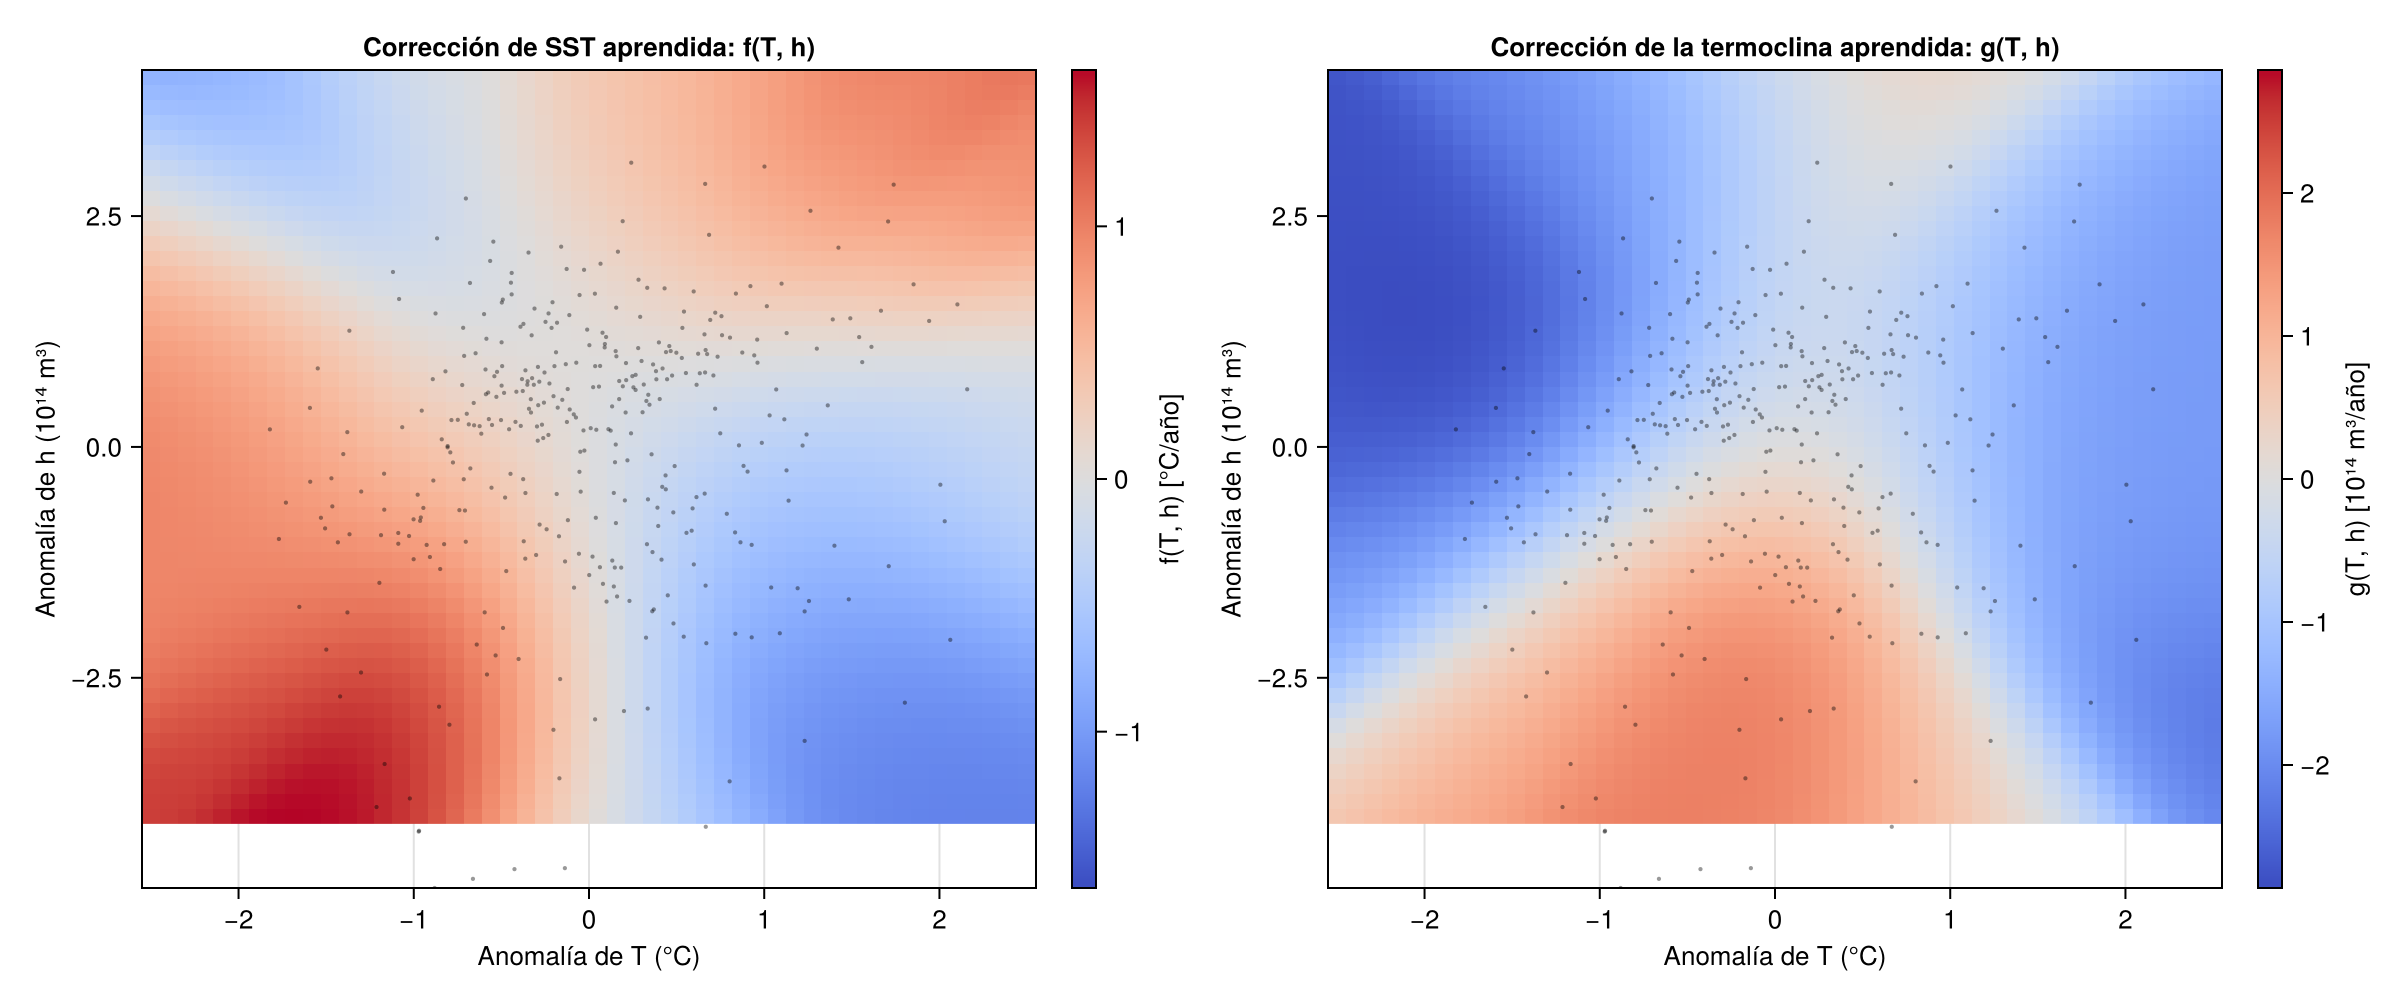
\includegraphics[width=0.95\textwidth]{figures/03_ude_nn_corrections.png}
\caption{Correcciones de drift aprendidas: $f_\phi(T,h)$ (SST, izquierda) y $g_\phi(T,h)$ (termoclina, derecha). Los puntos negros representan los datos de entrenamiento.}
\label{fig:nn_corrections}
\end{figure}

Las correcciones exhiben estructura física interpretable:
\begin{itemize}
  \item $f_\phi(T,h)$ exhibe una estructura diagonal clara: valores positivos (calentamiento) en las regiones donde T y h tienen el mismo signo y valores negativos (enfriamiento) donde tienen signos opuestos. Este patrón es consistente con una corrección proporcional al producto $T \dot h$, que corresponde al término de acoplamiento no-lineal de Bjerknes no capturado por el esqueleto lineal de Jin. La red redescubrió sin supervisión explícita un mecanismo de retroalimentación conocido en la literatura oceanográfica. Como en toda corrección neuronal, esta interpretación es una hipótesis plausible consistente con la física conocida, no una demostración de causalidad.
  \item $g_\phi(T,h)$ exhibe una franja de valores positivos centrada en $T \approx 0$, con valores negativos a ambos lados para anomalías grandes de SST. Este patrón es consistente con una corrección proporcional a $-|T|$, que actúa como una saturación no lineal en la tasa de recarga de la termoclina: el modelo lineal de Jin sobreestima la descarga de $h$ durante eventos extremos de SST, y la red corrige ese exceso. La leve inclinación de la franja sugiere una dependencia secundaria en $h$, posiblemente capturando asimetrías entre El Niño y La Niña en la dinámica de recarga. Como en toda corrección neuronal, esta interpretación es una hipótesis plausible consistente con la física conocida, no una demostración de causalidad.
\end{itemize}

\subsection{Evaluación fuera de muestra (2011--2021)}
\label{sec:oos}

La evaluación principal de habilidad predictiva se basa en pronósticos rodantes (\textit{rolling forecasts}) con re-inicialización, donde el modelo asimila el estado observado en cada instante $t$ para predecir $t+H$. La correlación decae gradualmente con el horizonte de predicción, como se espera en un sistema caótico (Figura~\ref{fig:skill_score}). El modelo BUSDE mantiene $r > 0.5$ hasta $H \approx 6$ meses, superando al OLS, a la componente lineal y a los baselines estándar (persistencia y climatología) en todos los horizontes evaluados.

\begin{figure}[H]
\centering
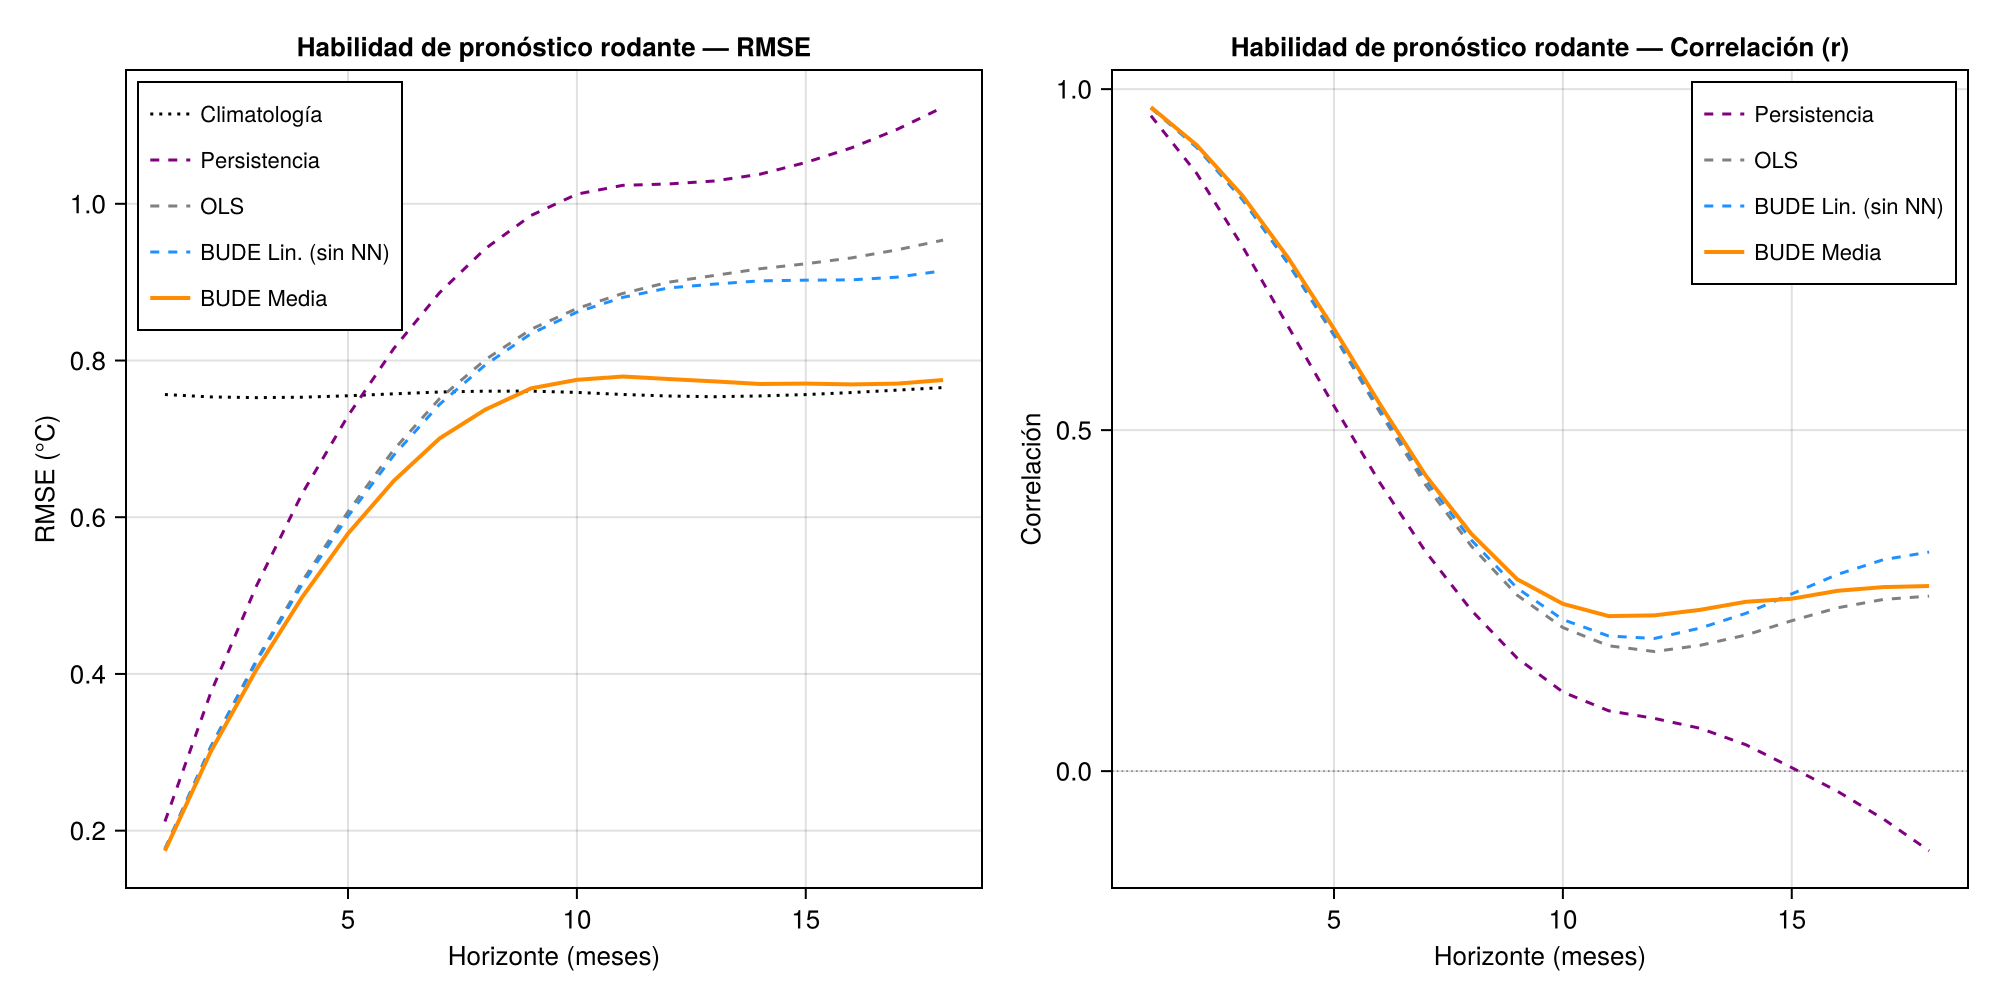
\includegraphics[width=0.95\textwidth]{figures/04_skill_score_bayesian.png}
\caption{RMSE y correlación de pronósticos rodantes en función del horizonte $H$ (1--18 meses), comparando BUSDE, componente lineal (sin NN), OLS, persistencia y climatología.}
\label{fig:skill_score}
\end{figure}

Como prueba adicional de \textbf{estabilidad del atractor}, la Figura~\ref{fig:test_rollout} presenta los rollouts determinísticos de integración continua sobre el periodo de prueba. El ensamble BUSDE alcanza $r = 0.203$ en un rollout libre de 11 años. Si bien esta correlación modesta a tan largo plazo no debe interpretarse como habilidad predictiva operativa, demuestra empíricamente que la climatología simulada se mantiene estructuralmente acotada y estable, superando a la divergencia de la componente lineal aislada ($r = -0.188$). La banda del 10--90\% del ensamble proporciona una cuantificación visual de la incertidumbre epistémica.

\begin{figure}[H]
\centering
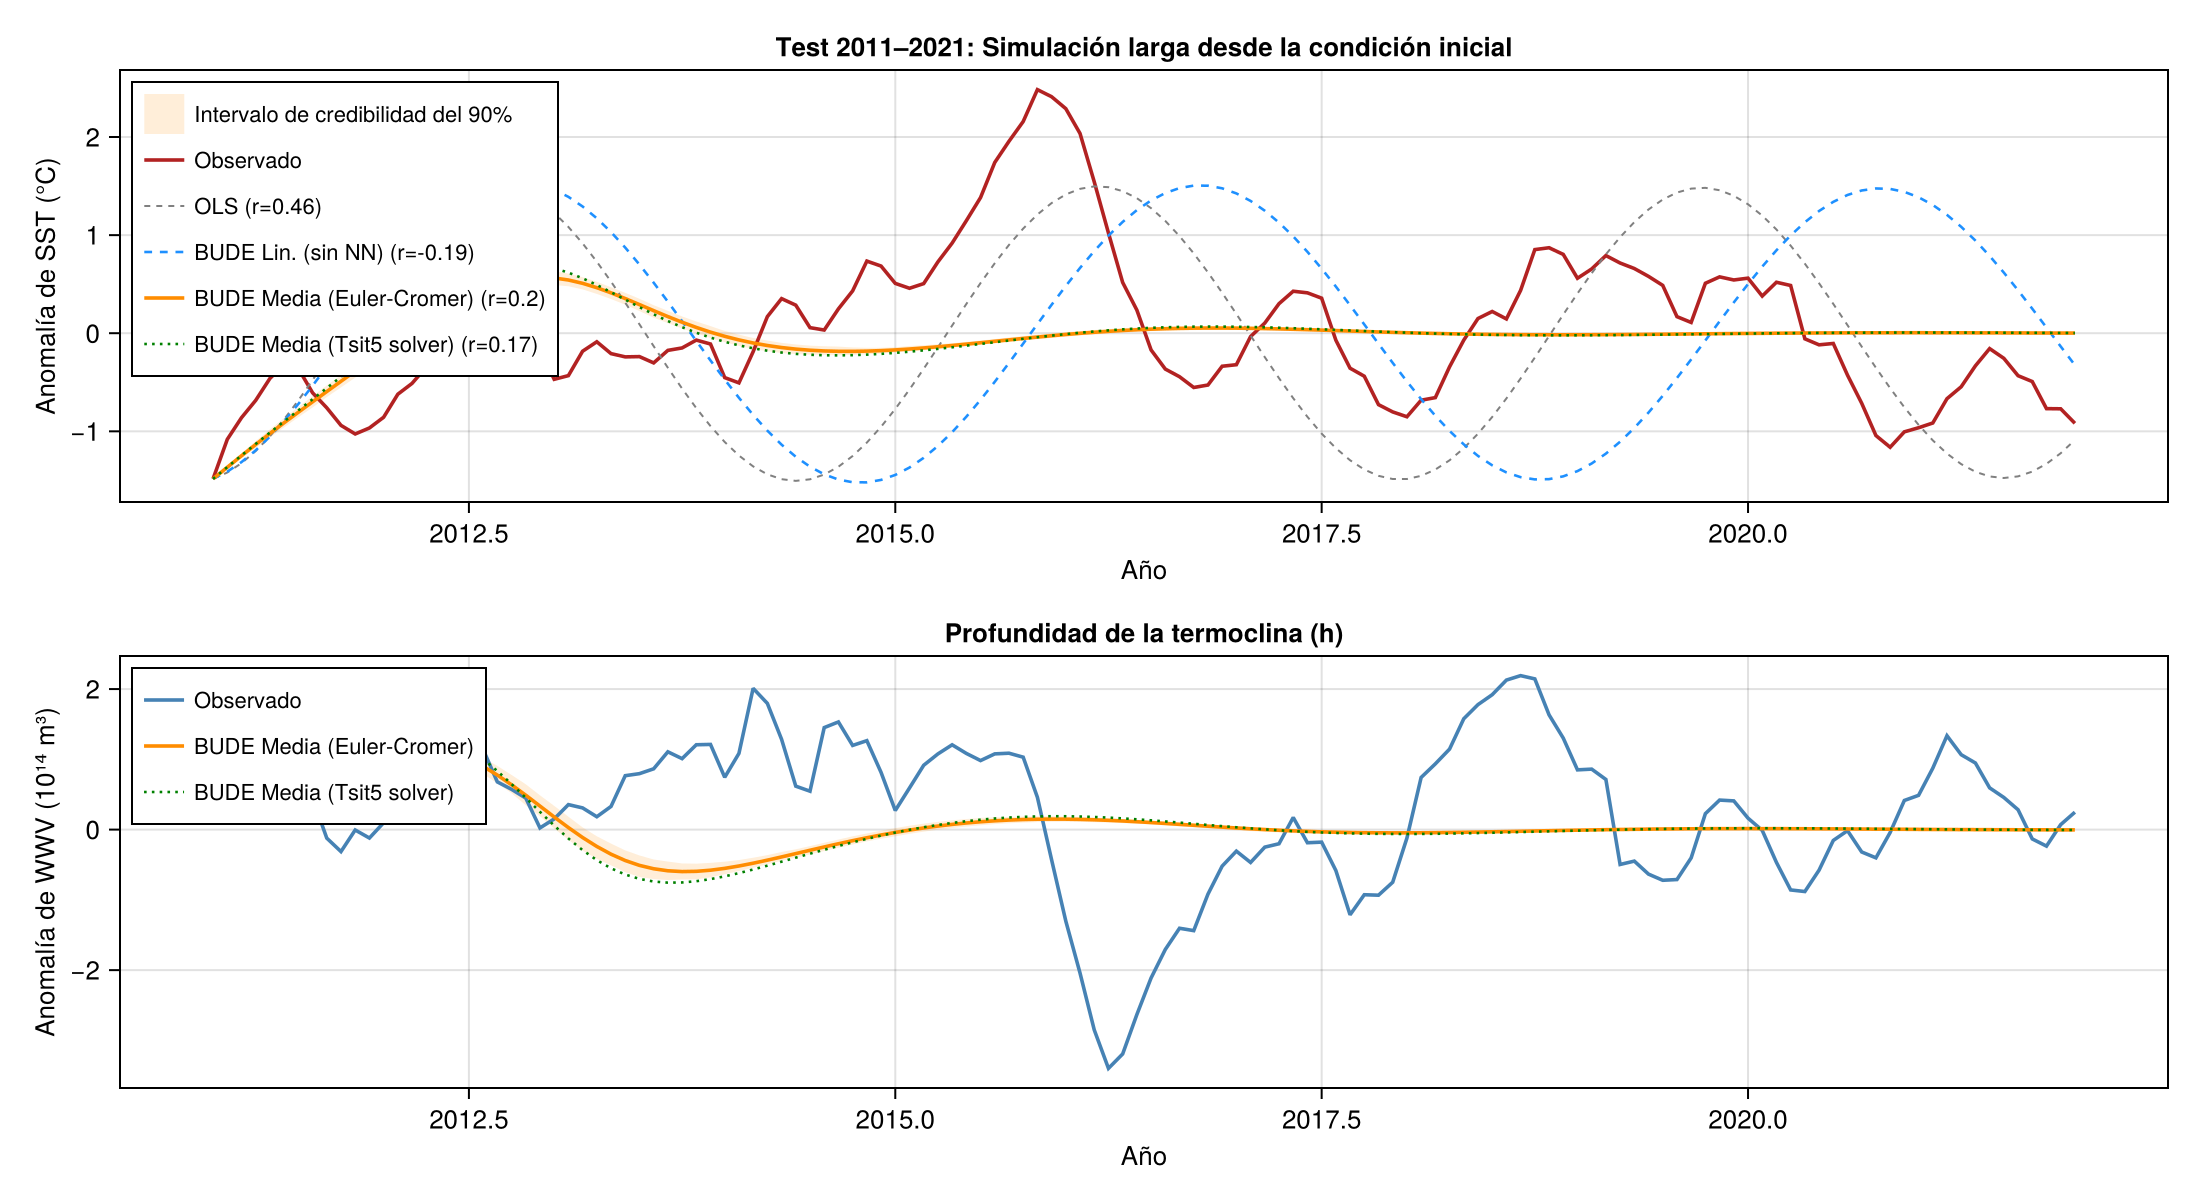
\includegraphics[width=0.95\textwidth]{figures/04_test_rollout_bayesian.png}
\caption{Rollout sobre el periodo de prueba (2011--2021) evaluando la estabilidad a largo plazo. Panel superior: SST. Panel inferior: WWV. Las bandas sombreadas representan el intervalo 10--90\% del ensamble bayesiano.}
\label{fig:test_rollout}
\end{figure}

\subsection{Modelo de ruido y dinámica a largo plazo}

Los residuos de predicción a un paso revelan una estructura de ruido significativa. El modelo heteroscedástico ajustado por MLE (Ec.~\ref{eq:hetero}) produce los coeficientes $\gamma_T = [-0.408,\; 0.055,\; -0.080]$ para el ruido de SST ($T$), y $\gamma_h = [0.345,\; 0.150,\; -0.021]$ para el ruido de la termoclina ($h$). Cabe destacar que el término de difusión estocástica actúa matemáticamente como un residuo agregado que captura toda la dinámica no representada por la deriva (incluyendo escalas temporales subdiarias, forzamiento atmosférico de alta frecuencia, errores de observación y aproximaciones numéricas del modelo conceptual). Bajo esta perspectiva, las asociaciones físicas sugeridas por los coeficientes deben interpretarse con cautela como hipótesis plausibles y no como demostraciones de causalidad directa:
\begin{itemize}
  \item El coeficiente positivo $\gamma_{T,1} = 0.055 > 0$ indica empíricamente que la intensidad del residuo en SST aumenta cuando la anomalía de temperatura es positiva. Esto es consistente con la hipótesis climática de que las anomalías cálidas de SST favorecen una mayor actividad de ráfagas de viento del oeste (\textit{Westerly Wind Bursts}) que inyectan energía estocástica al océano \citep{eisenman2005}.
  \item El coeficiente negativo $\gamma_{T,2} = -0.080 < 0$ indica que una termoclina somera ($h < 0$, fase de descarga de calor) se asocia a una mayor variabilidad residual en SST. Esto condice con la sensibilidad física de la retroalimentación de la termoclina: al estar más cerca de la superficie, fluctuaciones atmosféricas no resueltas de alta frecuencia impactan de forma más directa y rápida sobre la temperatura superficial.
  \item El coeficiente positivo $\gamma_{h,1} = 0.150 > 0$ muestra que la variabilidad estocástica en la tasa de cambio de la termoclina aumenta ante anomalías cálidas de SST. Esto sugiere que las perturbaciones de viento zonales que fuerzan la dinámica del océano ecuatorial podrían ser más activas o variables cuando el sistema está en un estado acoplado cálido.
\end{itemize}

La Figura~\ref{fig:noise_surface} visualiza esta superficie de ruido de SST dependiente del estado. El mapa exhibe un claro gradiente diagonal, con los valores máximos concentrados en la esquina inferior derecha (SST cálida y termoclina somera). Esta configuración es característica de la fase de terminación de El Niño, sugiriendo que la irregularidad en el fin de estos eventos está condicionada por la amplificación de perturbaciones estocásticas no resueltas en esta región del espacio de fases.



\begin{figure}[H]
\centering
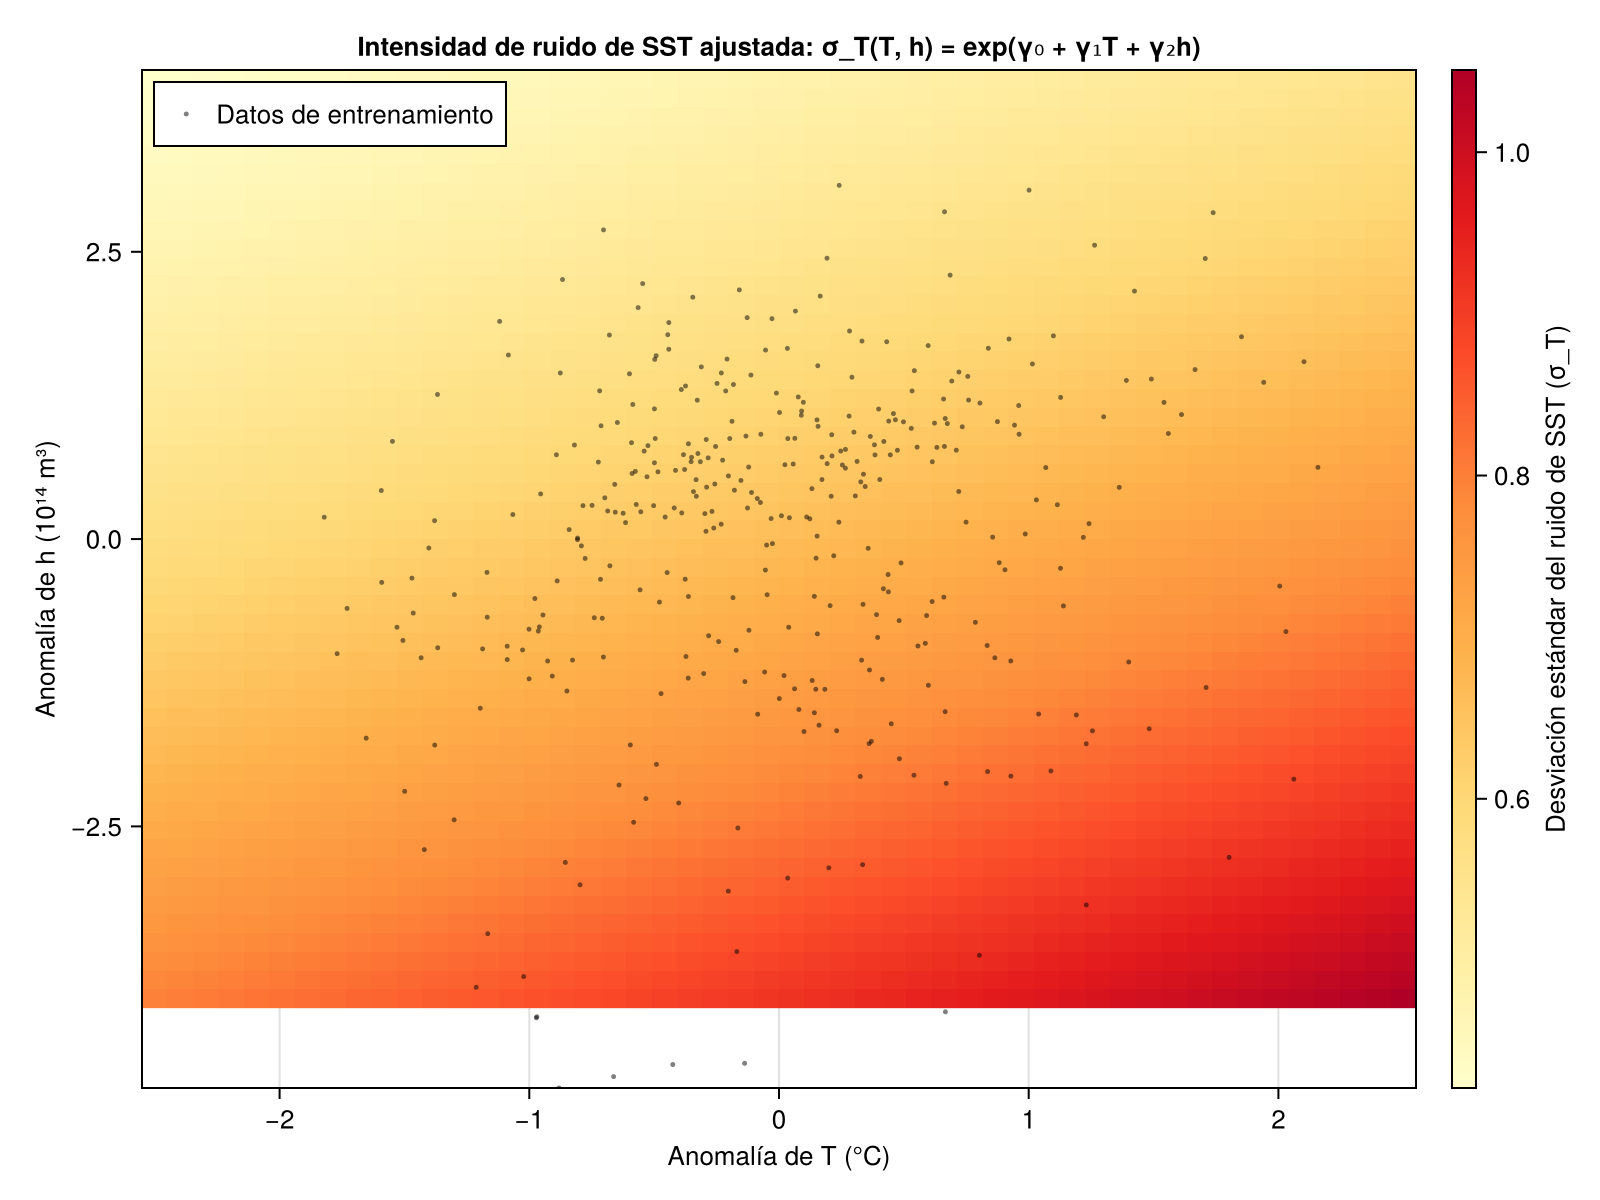
\includegraphics[width=0.6\textwidth]{figures/05_noise_surface.png}
\caption{Intensidad del ruido SST ajustada: $\sigma_T(T, h) = \exp(\gamma_0 + \gamma_1 T + \gamma_2 h)$.}
\label{fig:noise_surface}
\end{figure}

Las simulaciones SDE de 500 años con el modelo de drift BUSDE permiten analizar la dinámica de largo plazo del sistema. Tanto el SDE homoscedástico como el heteroscedástico producen distribuciones de intervalos inter-evento con CV más cercano a las observaciones históricas que los modelos estocásticos nulos (persistencia con ruido y OLS con ruido homocedástico), demostrando que la estructura BUSDE captura cualitativamente mejor la irregularidad del ENSO (Figura~\ref{fig:sde_analysis}).

\begin{figure}[H]
\centering
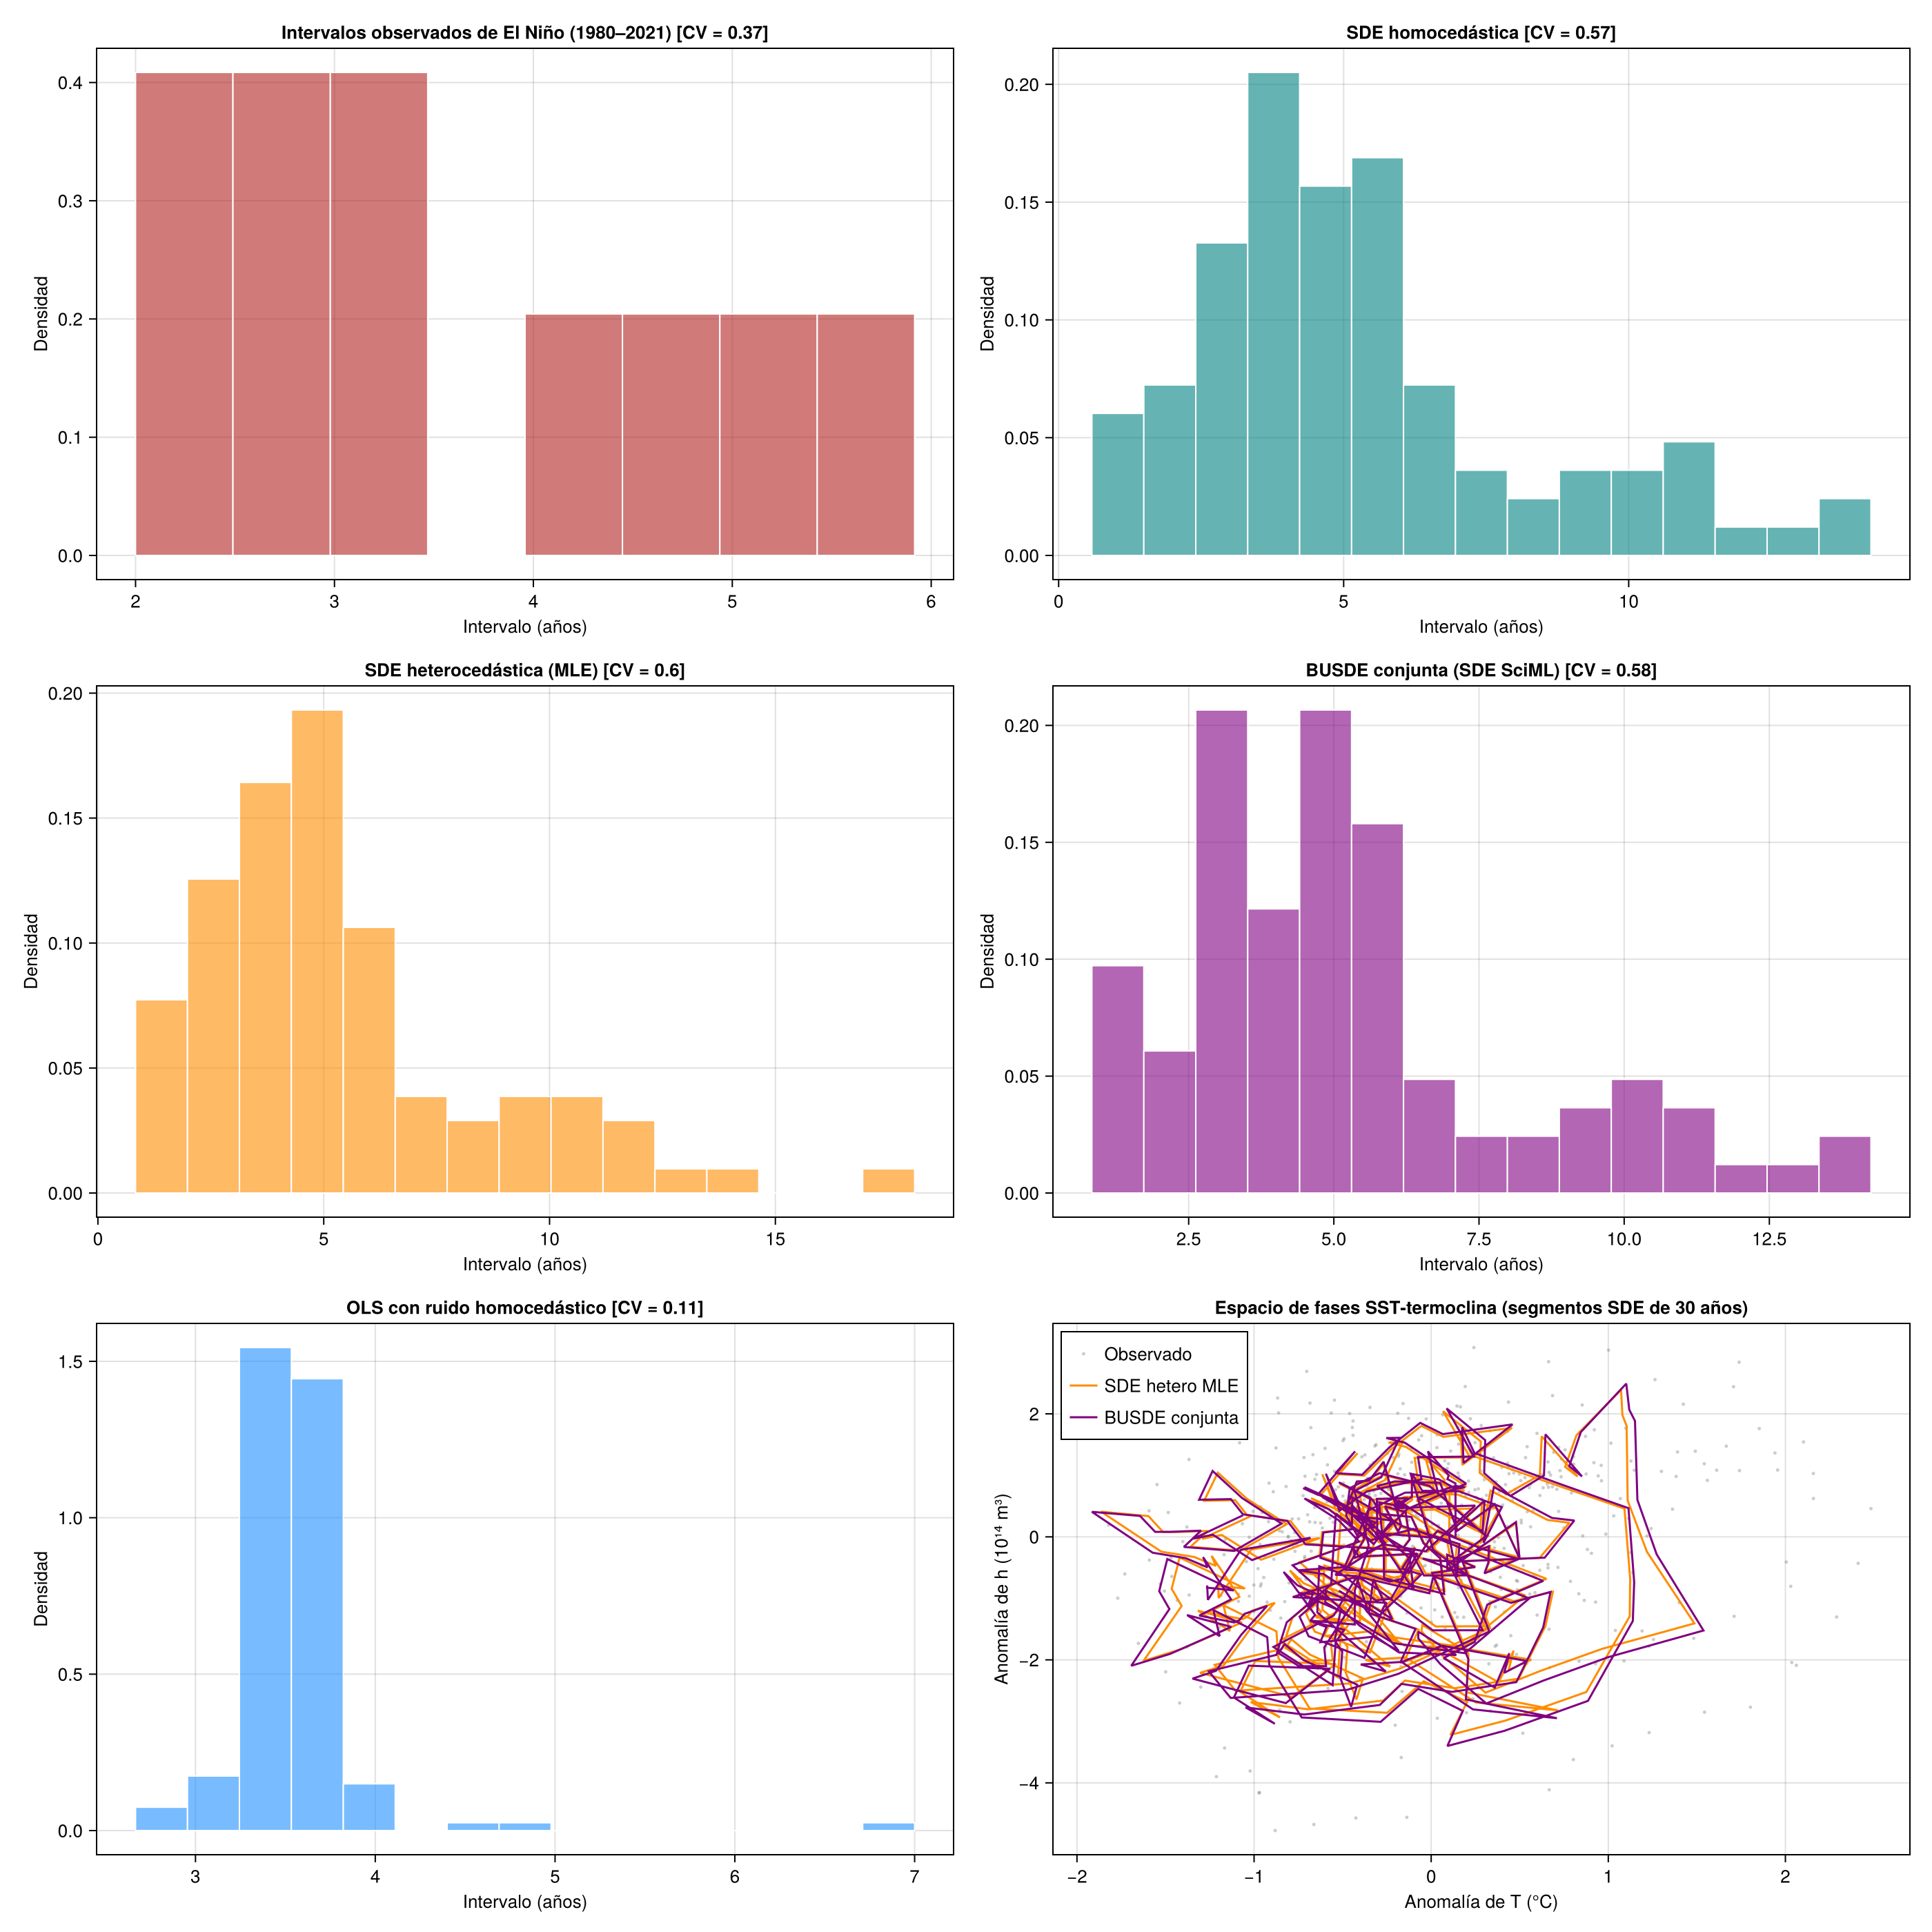
\includegraphics[width=0.85\textwidth]{figures/05_sde_analysis.png}
\caption{Análisis de largo plazo: distribuciones de intervalos inter-evento comparando observaciones y baselines estocásticos (OLS, Persistencia) contra las simulaciones de la BUSDE heterocedástica.}
\label{fig:sde_analysis}
\end{figure}

\subsection{Verificación probabilística}

En la Figura \ref{fig:verification} se presentan los resultados de la verificación probabilística fuera de muestra utilizando $M = 1000$ realizaciones del ensamble conjunto (incertidumbre paramétrica + estocástica).

Se observa que el CRPS del modelo es muy inferior al baseline climatológico para horizontes menores a 7.5 meses, indicando alta habilidad a corto plazo.
La cobertura del intervalo de predicción al 90\% es cercana al valor nominal para horizontes cortos (1 o 2 meses) y cae rapidamente. El modelo está subdisperso a horizontes largos.


\begin{figure}[H]
\centering
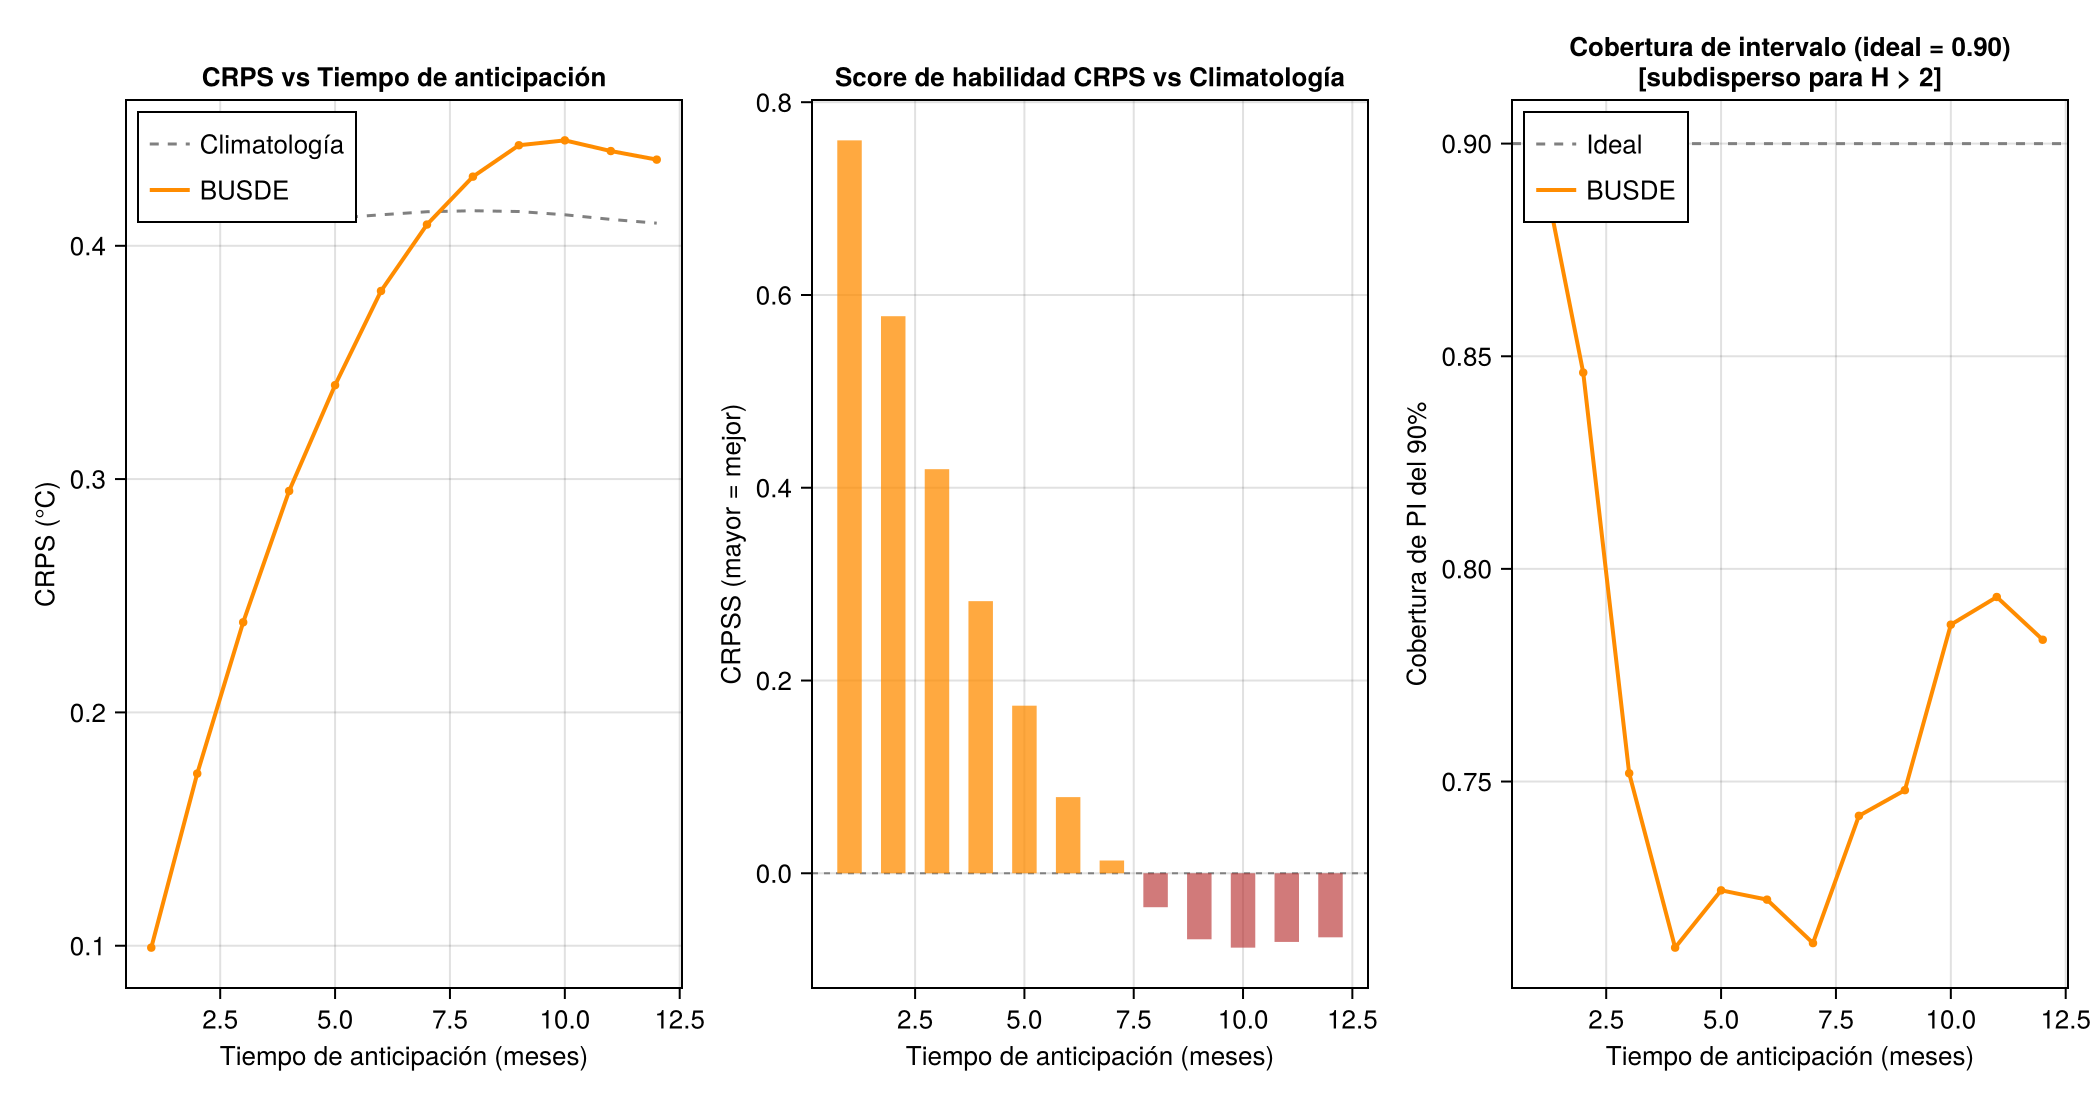
\includegraphics[width=0.95\textwidth]{figures/06_verification_scores.png}
\caption{Verificación probabilística: (a) CRPS vs.\ horizonte, (b) CRPS Skill Score vs.\ climatología, (c) cobertura del intervalo de predicción al 90\%.}
\label{fig:verification}
\end{figure}




\subsection{Comparación BUDE vs.\ BUSDE}

Para cuantificar la contribución del ruido estocástico a la calibración probabilística, se comparó el modelo BUDE (solo incertidumbre epistémica, sin término de difusión) con el modelo completo BUSDE (incertidumbre epistémica + aleatoria). En la Figura \ref{fig:budevsbusde} se puede ver que el modelo BUDE produce intervalos de predicción severamente \textbf{subdispersados}: la cobertura del 90\% cae por debajo del 50\% para $H > 3$ meses, dado que la incertidumbre epistémica sola es insuficiente.


El modelo BUSDE mejora sustancialmente la calibración en todos los horizontes, con coberturas más cercanas al valor nominal.

El CRPS del BUSDE es consistentemente inferior (mejor) al del BUDE en horizontes $H > 1$ mes.


Esta comparación demuestra que el término de difusión estocástica es un componente esencial del marco predictivo, no un accesorio opcional.


\begin{figure}[H]
\centering
\includegraphics[width=0.85\textwidth]{figures/10_bude_vs_busde.png}
\caption{Comparación BUDE vs BUSDE. (A)CRPS vs. horizonte, (B) Cobertura del intervalo de predicción al 90\%, (C) Confiabilidad a 6 meses, (D) Abanico a 12 meses}
\label{fig:budevsbusde}
\end{figure}


% ============================================================================
% 4. DISCUSIÓN Y CONCLUSIONES
% ============================================================================

\section{Discusión y conclusiones}
\label{sec:discusion}

\subsection{Contribuciones principales}

Este trabajo presenta un marco integrado BUSDE que combina principios físicos, aprendizaje automático y estadística bayesiana para modelar la dinámica del ENSO. Las principales contribuciones son:

\begin{enumerate}
  \item \textbf{Correcciones neuronales interpretables:} Las redes neuronales $f_\phi$ y $g_\phi$ aprenden dinámicas físicamente coherentes, incluyendo el amortiguamiento convectivo no-lineal a altas temperaturas y la descarga asimétrica de la termoclina. Estos patrones son consistentes con la literatura oceanográfica y demuestran el potencial de las UDE como herramienta de descubrimiento científico.

  \item \textbf{Incertidumbre cuantificada:} La inferencia variacional proporciona distribuciones posteriores sobre todos los parámetros del modelo, permitiendo la generación de pronósticos probabilísticos que combinan incertidumbre epistémica y aleatoria. A $H = 1$ mes, la cobertura del intervalo de predicción al 90\% es de 90.1\%, prácticamente idéntica al valor nominal.

  \item \textbf{Evidencia empírica de acoplamiento WWB:} El modelo de ruido heteroscedástico revela un coeficiente positivo $\gamma_{T,1} > 0$ en la intensidad del ruido SST, consistente con la hipótesis de acoplamiento entre anomalías cálidas y ráfagas de viento del oeste. Dado que el término de difusión captura toda la dinámica no representada por el drift - incluyendo errores de modelo y aproximaciones numéricas - esta asociación debe interpretarse como una hipótesis plausible y no como evidencia causal directa \citep{eisenman2005}.

  \item \textbf{Estabilidad de largo plazo:} El modelo BUSDE produce simulaciones SDE numéricamente estables durante 500+ años, con estadísticas de ciclo (frecuencia, irregularidad) cualitativamente consistentes con las observaciones históricas.
\end{enumerate}

\subsection{Limitaciones}

Identificamos tres limitaciones importantes que deben contextualizarse:

\paragraph{Subdispersión a horizontes largos.} La cobertura del intervalo de predicción cae sistemáticamente por debajo del valor nominal para $H > 2$ meses, llegando a un déficit del 17\% a $H = 6$. Esto ocurre porque el SDE markoviano de Itô, al calibrar su intensidad de ruido exclusivamente con residuos a un paso ($\Delta t = 1/12$), es estructuralmente ciego al crecimiento exponencial de Lyapunov de los errores caóticos a horizontes largos ($H \gg \Delta t$). Para corregir esta limitación fundamental, el trabajo futuro debería explorar dinámicas con memoria, como ecuaciones de Langevin Generalizadas, para representar correctamente el forzamiento estocástico acumulado.

\paragraph{Co-optimización de parámetros.} Los coeficientes lineales $(a, b, c)$ se optimizan conjuntamente con los pesos neuronales. Esto implica que no pueden interpretarse como constantes físicas independientes del Oscilador de Recarga aislado. Cualquier análisis que extraiga los parámetros lineales sin las correcciones neuronales correspondientes incurre en un \textit{model mismatch} severo.

\paragraph{Ventana de evaluación limitada.} El periodo de prueba de 11 años (2011--2021) contiene solo $\approx 2.5$ ciclos ENSO completos, lo que limita la robustez estadística de las métricas fuera de muestra. En particular, las conclusiones sobre habilidad predictiva a escalas interanuales deben interpretarse con cautela.



\subsection{Trabajo futuro}

Líneas prometedoras de extensión incluyen: (i) la incorporación de un modelo de ruido multiplicativo que escale con el horizonte de predicción para corregir la subdispersión residual; (ii)~la extensión a modelos con más variables de estado (e.g., viento zonal, precipitación) para mejorar la resolución de los procesos no representados; (iii)~la aplicación de técnicas de asimilación de datos en tiempo real para actualizar la distribución posterior conforme se dispone de nuevas observaciones; y (iv)~el uso de funciones de base más expresivas (redes residuales profundas, transformadores) para capturar dinámicas de mayor complejidad.

% ============================================================================
% 5. AGRADECIMIENTOS
% ============================================================================





\section*{Agradecimientos}

Este trabajo se desarrolló con asistencia de Claude (Anthropic) para la revisión del código, la depuración de errores y la generación de borradores de texto. Todas las decisiones científicas, la interpretación de resultados y la redacción final fueron responsabilidad del autor.

% ============================================================================
% 6. DATOS Y SOFTWARE
% ============================================================================
\section*{Datos y Software}

Las anomalías de temperatura superficial del mar (SST) se obtuvieron del dataset público ERSSTv5 (\textit{Extended Reconstructed Sea Surface Temperature}, versión 5) de NOAA, disponible en \url{https://www.ncei.noaa.gov/products/extended-reconstructed-sst} \citep{huang2017}. El índice de Volumen de Agua Caliente (WWV) se obtuvo del NOAA Pacific Marine Environmental Laboratory (PMEL), disponible en \url{https://www.pmel.noaa.gov/tao/wwv/}.

El código desarrollado para este proyecto está disponible en el \href{https://github.com/mathyrolando/BUSDE-ENSO}{repositorio GitHub}. Este proyecto fue desarrollado en Julia v1.12.5 utilizando los siguientes paquetes principales: DifferentialEquations.jl \citep{rackauckas2017}, Lux.jl \citep{lux2022}, Zygote.jl (diferenciación automática), ComponentArrays.jl, Optimisers.jl (Adam), Optim.jl (Nelder-Mead), CairoMakie.jl (visualización), JLD2.jl y CSV.jl (serialización de datos). Las versiones exactas de todas las dependencias se encuentran fijadas en el archivo \texttt{Manifest.toml} del repositorio. El código fuente del proyecto se encuentra disponible en el repositorio del curso.

% ============================================================================
% 7. REFERENCIAS
% ============================================================================
\bibliographystyle{plainnat}
\bibliography{referencias}

\end{document}
